%!TEX program = xelatex
\documentclass[12pt, a4paper]{article}

% --- PACOTES BÁSICOS E GEOMETRIA ---
\usepackage[a4paper, top=3cm, bottom=2cm, left=3cm, right=2cm]{geometry}
\usepackage{fontspec}
\usepackage[brazilian]{babel}
\usepackage{microtype} % Melhora o ajuste tipográfico

% --- FONTE SERIFADA E ELEGANTE ---
% Utiliza a Noto Serif (disponível por padrão no ambiente XeLaTeX/LuaLaTeX)
\babelfont{rm}{Noto Serif}

%---- Pacotes Gráficos ------
\usepackage{float}
\usepackage{graphicx}
\graphicspath{{./src/img/}}

%------ HYPERLINKS ------------
\usepackage{hyperref}
\hypersetup{
    colorlinks=true, % Ativa a cor nos links (em vez do retângulo em volta)
    linkcolor=blue, % Cor dos links internos (como sumário ou referências)
    urlcolor=blue % Cor dos hyperlinks externos (URLs)
}

% --- ESPAÇAMENTO E RECUO DE PARÁGRAFO ---
\usepackage{setspace}
\onehalfspacing % Espaçamento de 1,5 entre linhas
\setlength{\parindent}{1.25cm} % Indentação padrão dos parágrafos
\setlength{\parskip}{0pt}       % Sem espaçamento extra entre parágrafos (mantém padrão acadêmico/elegante)

% --- PALETA DE CORES EM TONS PASTÉIS ---
\usepackage[table]{xcolor}
% Definição das cores em tons pastéis
\definecolor{pastelPrimary}{RGB}{74, 98, 116}    % Azul acinzentado suave para títulos
\definecolor{pastelSecondary}{RGB}{115, 147, 126}% Verde salvia suave
\definecolor{pastelBgNote}{RGB}{245, 247, 248}   % Fundo cinza/azul claríssimo
\definecolor{pastelBorderNote}{RGB}{180, 196, 201} % Borda pastel para observações
\definecolor{pastelQuoteBg}{RGB}{250, 246, 240}  % Fundo bege pastel quente
\definecolor{pastelQuoteBar}{RGB}{212, 180, 150} % Borda terracota pastel
\definecolor{pastelText}{RGB}{45, 55, 65}        % Texto principal em cinza escuro elegante

% Aplica cor ao texto normal para evitar o preto absoluto muito rígido
\color{pastelText}

% --- ESTILIZAÇÃO DOS TÍTULOS ---
\usepackage{titlesec}
\titleformat{\section}
  {\Large\bfseries\color{pastelPrimary}}
  {\thesection}{1em}{}
  [\color{pastelBorderNote}\rule{\textwidth}{0.6pt}]

\titleformat{\subsection}
  {\large\bfseries\color{pastelSecondary}}
  {\thesubsection}{1em}{}

% --- CAIXAS DE OBSERVAÇÃO E CITAÇÃO (TCOLORBOX) ---
\usepackage[many]{tcolorbox}

% 1. Caixa de Observação
\newtcolorbox{observacao}[1][Observação]{
  enhanced,
  breakable,
  colback=pastelBgNote,
  colframe=pastelBorderNote,
  fonttitle=\bfseries\color{pastelPrimary},
  title={#1},
  title style={draw=none, fill=none},
  lefttitle=0pt,
  top=8pt,
  bottom=8pt,
  left=12pt,
  right=12pt,
  arc=3pt,
  boxrule=0.8pt,
  parbox=false,
  before upper={\setlength{\parindent}{1.25cm}} % Preserva indentação interna
}

% 2. Caixa de Citação Destacada
\newtcolorbox{citacaodestaque}[1][]{
  enhanced,
  breakable,
  colback=pastelQuoteBg,
  frame hidden,
  borderline west={3.5pt}{0pt}{pastelQuoteBar},
  arc=0pt,
  outer arc=0pt,
  top=10pt,
  bottom=10pt,
  left=14pt,
  right=10pt,
  parbox=false,
  fontupper=\itshape\color{pastelText},
  #1
}

% --- DADOS DO DOCUMENTO ---
\title{\Huge\bfseries\color{pastelPrimary} Logaritmos e Escalas Logarítmicas}
\author{\Large\color{pastelSecondary} Anne Michle}
\date{\large \today}

\begin{document}

\maketitle

\section{Terremoto!}

O conhecimento científico que se desenvolve sobre terremotos faz com que os danos, mesmo em abalos de altíssima magnitude, sejam muito menores do que aqueles decorrentes de terremotos mais fracos em situações em que as tecnologias não figuravam no quadro. Então vamos aprender um pouquinho sobre o assunto e sobre o que a matemática tem a ver com isso.

No Brasil, felizmente, terremotos são raros e quando ocorrem não costumam ser fortes (devido à situação geológica do terreno sobre o qual vivemos). Mas aqui mesmo na América do Sul, no Chile (que geologicamente não está em uma área tão estável quanto a nossa), ocorrem tremores de terra com frequência. No dia 16 de setembro de 2015 ocorreu um grande terremoto, que atingiu 8,3 graus na escala Richter. Para dar uma ideia do que significa isso, sugiro que dêem uma olhada no vídeo de 3 minutos cujo link segue abaixo. Ele nos permite perceber o quanto a terra pode tremer e o quão assustador pode ser isso.

\vspace{0.8em}

\begin{observacao}[Jornal da Globo - Terremoto do Chile - 16.09.2015]
  \href{https://globoplay.globo.com/v/4472903/}{Clique aqui para acessar o recurso}. Dê uma olhada nesta notícia e veja o vídeo de 3 minutos. Veja como a terra treme com um terremoto de 8.3 graus (segunda metade do vídeo traz imagens e depoimentos).
\end{observacao}

\vspace{0.8em}

A magnitude de um terremoto na escala Richter é obtida por um cálculo (envolvendo logaritmos) realizado sobre a amplitude das vibrações sísmicas medida pelo sismógrafo. Pelas ilustrações abaixo você pode ter uma ideia de como um sismógrafo realiza estas medições.

\begin{figure}
  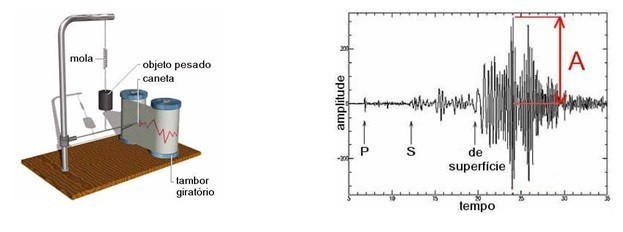
\includegraphics[width=.8\textwidth]{sismografo.jpg}
  \caption{imagens do site Física Moderna}
\end{figure}

Essencialmente, podemos obter a magnitude M de um terremoto, dividindo a amplitude A registrada no sismógrafo por uma amplitude de referência $A_0$ e extraindo o logaritmo na base $10: M = \log _{10} (A/ A_{0})$. 
Então, quando $M = 8,3$ graus nesta escala, significa que a amplitude A medida no sismógrafo é $10^{8.3} A_0$, isto é, aproximadamente $200$ milhões de vezes a variação sísmica de referência $A_0$ (pois $10^{8.3} =199.526.231,5$).


\section{Comparando Terremotos}

Nosso objetivo ao tratar dos terremotos é entender porque os logaritmos são indispensáveis para mensurar este fenômeno. Para perceber a necessidade destas (muitas vezes incompreendidas) funções matemáticas, vamos tentar comparar aproximações para os valores $A/A_0$ obtidas a partir das observações dos sismógrafos (sem fazer uso dos logaritmos). O que significa $A/A_0$? Esse valor nos diz quantas vezes maior a amplitude registrada no sismógrafo é em relação à amplitude de referência. Vejamos...

\vspace{0.6em}

\begin{figure}[H]
  \centering
  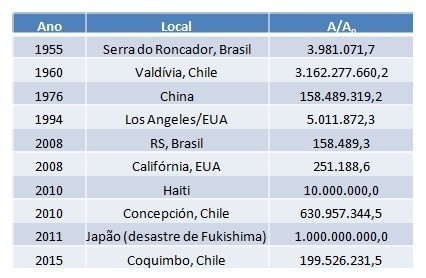
\includegraphics[width=.65\textwidth]{tabela_terremotos.png}
\end{figure}

\vspace{0.6em}

Dê uma olhada nos números da coluna da direita... O que você percebe? Podemos ver que o maior número corresponde ao terremoto de 1960, no Chile, sendo maior que 3 bilhões. Já o menor nesta tabela é o do Brasil em 2008, próximo a 160 mil (este dado está aí para termos como referência alguma medição recente em nosso país). Mas com números tão díspares é difícil perceber a relação entre eles. Vamos usar nossa principal ferramenta para este tipo de tarefa: um gráfico.

No gráfico usamos para o eixo y uma escala que mostra valores de 0 a 6 milhões. Veja que com essa escala só podemos ver no gráfico 4 dos 10 terremotos da tabela. Você deve tentar mudar a escala, mexendo na barra de controle que aparece no gráfico de forma a tentar visualizar simultaneamente e comparar os pontos correspondentes aos 10 terremotos registrados na tabela acima. 

\vspace{0.8em}

\begin{observacao}[Applet Geogebra]
  \href{https://www.geogebra.org/m/uca9armn}{Comparador de intensidades de terremotos}.
\end{observacao}

\vspace{0.8em}

Você consegue comparar através deste gráfico as intensidades dos terremotos do Brasil simultaneamente com os chilenos e o japonês?

Não, provavelmente, não...

Você deve ter observado que é impossível comparar neste gráfico a intensidade destes 10 terremotos. Como a variação entre as intensidades é muito grande, quando a escala permite que vejamos os mais intensos, os mais fracos desaparecem no eixo x. E se mudarmos a escala de forma que se possa ver as diferenças entre os mais fracos, os mais intenso não se encaixarão na área visível.

Qual a solução?

Escala logarítmica! Em vez de olhar os valores $A/A_0$, faremos como propôs Richter e seus colaboradores: usamos os logaritmos destes valores! Veja como fica:

\begin{figure}[H]
  \centering
  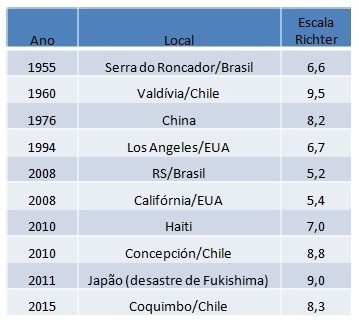
\includegraphics[width=.45\textwidth]{tabela_richter.jpg}
\end{figure}

Agora, temos na tabela $\log _10 (A/A_0)$ para cada terremoto e podemos comparar facilmente estes valores em um mesmo gráfico.

\vspace{0.8em}

\begin{figure}[H]
  \centering
  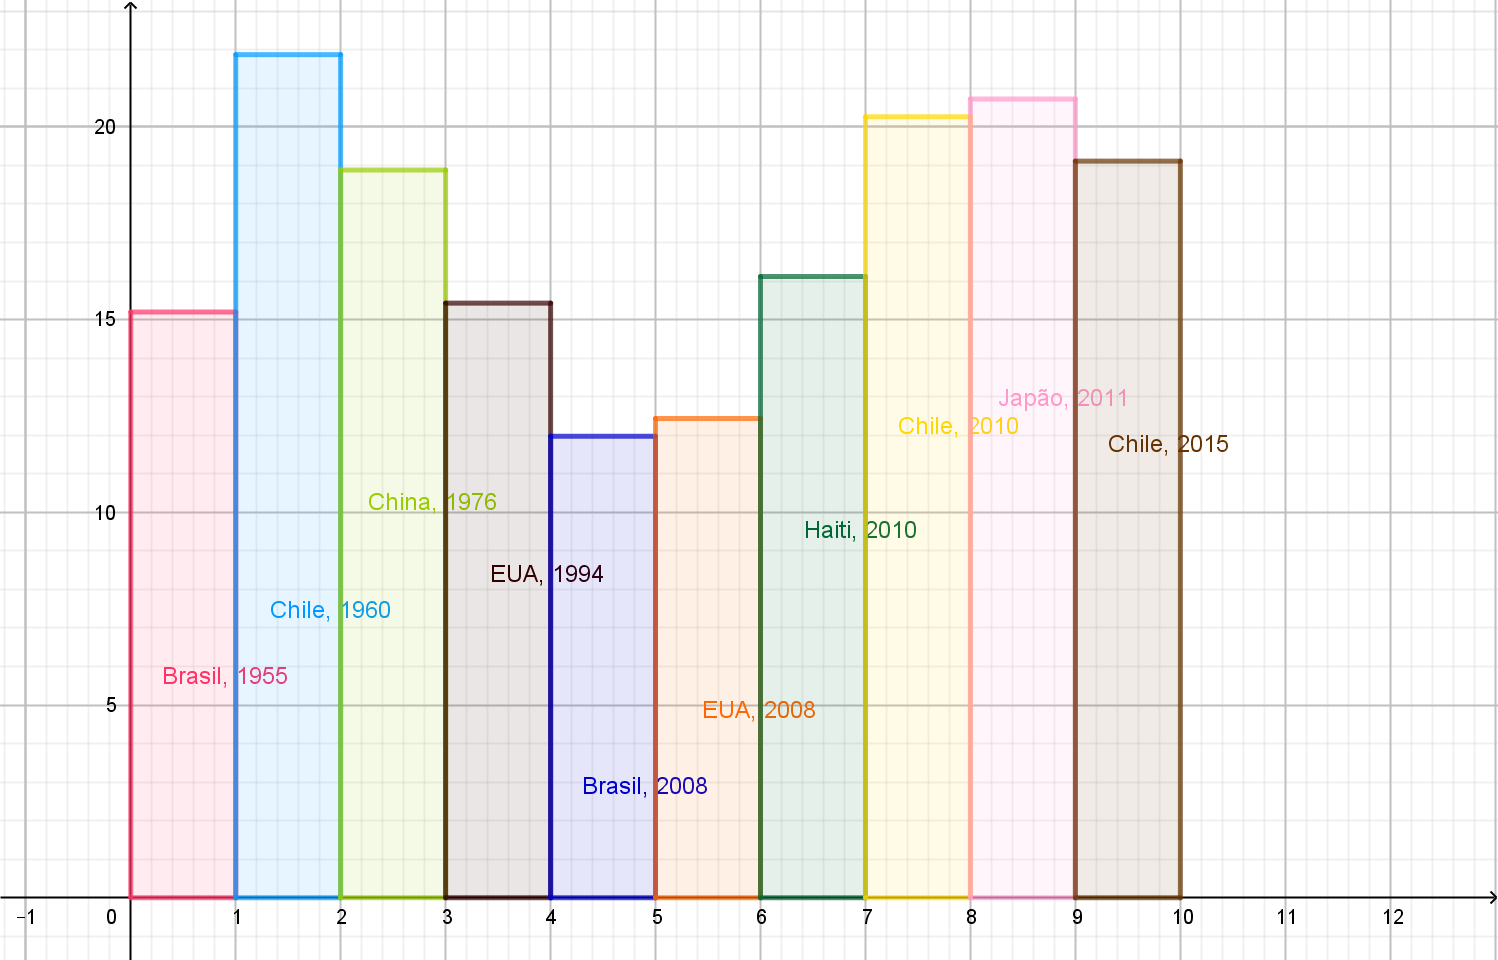
\includegraphics[width=.6\textwidth]{grafico_richter.png}
\end{figure}

\vspace{0.8em}

Podemos ver, por exemplo, que o terremoto de 2015 no Chile foi realmente muito forte! Contudo, houve apenas 11 mortes, enquanto no terremoto do Haiti, consideravelmente mais fraco, houve mais de 100 mil mortos. O número reduzido de fatalidades, no caso do Chile, se deve sobretudo às medidas preventivas como construções mais resistentes a abalos, já que o país é constantemente sacudido por terremotos. 

\begin{observacao}
  Com a atividade que realizamos até aqui você deve ter entendido porque é realmente necessário usar logaritmos para modelar fenômenos em que as variações ocorrem em ordens de grandeza muito diferentes ou em que há crescimento de ordem exponencial. Observe o quanto foi importante que você mesmo tentasse acertar a escala no primeiro gráfico para se convencer de que era necessário algum outro método para visualizar e comparar os terremotos em um gráfico. Sempre que você puder levar seus alunos ao laboratório para realizar experimentos matemáticos e aprenderem de forma ativa, deve fazê-lo.
\end{observacao}

\section{Um pouco mais sobre terremotos, escala Richter e logaritmos}

Agora vamos conhecer um pouco mais sobre o tema que estamos abordando.

O vídeo abaixo, produzido na Unicamp, é uma boa ferramenta para utilizar quando estiver ensinando logaritmo. Temos também o guia do professor associado ao vídeo. Assista o vídeo e dê uma olhada no guia do professor.

\begin{observacao}[Recurso didático: Terremoto Brasileiro]
  Vídeo para apoio ao ensino de logaritmo produzido na UNICAMP. Neste site você encontra o vídeo e ainda outras informações sobre este recurso pedagógico:

  \vspace{0.8em}

  \href{https://m3.ime.unicamp.br/recursos/1182}{Vídeo}

  \href{https://graduacao.cederj.edu.br/pluginfile.php/25005/mod_resource/content/1/terremotobrasileiro-guia.pdf}{Guia do Professor}
\end{observacao}

\subsection{Dos terremotos para a taxa de crescimento de funções}

De forma geral, logaritmo é um assunto temido e mal compreendido pelos alunos no ensino básico, para os quais o tema costuma parecer apenas um matematicismo caracterizado por um amontoado de regras, algo desnecessário no mundo real. As atividades sobre terremotos que propusemos até aqui têm por objetivo apresentar uma forma de levar o aluno a perceber porque as funções logarítmicas são realmente muito úteis e necessárias à aplicações práticas da matemática. Além disso, buscam também fornecer ao aluno compreensão sobre características qualitativas desta função (como o crescimento lento).

Do ponto de vista matemático, essa propriedade das escalas logarítmicas de nos permitir visualizar em uma escala única fenômenos que possuem comportamento exponencial ou variação com características de comportamento exponencial (como no caso da intensidade dos terremotos) se traduz no fato de que quando calculamos os logaritmos dos termos de uma progressão geométrica (algo que cresce exponencialmente) obtemos uma progressão aritmética (algo que cresce linearmente). Vamos estudar isso lendo a seção PG vira PA da Aula 24 dos cadernos didáticos:

\begin{observacao}[P.G. vira P.A.?]
  \href{https://graduacao.cederj.edu.br/pluginfile.php/25007/mod_resource/content/2/trecho%20aula%2024%20ieaa%20-%20PG%20vira%20PA.pdf}{Cadernos Didáticos, Vol. 3, p. 87}
\end{observacao}

Agora vamos explorar um pouco mais os aspectos qualitativos da função logarítmica trabalhando sobre seus gráficos e observando algumas características destes (como o crescimento lento). Para isso, vamos estudar a seção “A Função Logarítmica” da aula 24 (postada aqui com comentário e correção de erro tipográfico) e realizar outro experimento eletrônico que nos ajudará a conhecer melhor os gráficos deste tipo de função.

\begin{observacao}[Recurso Externo]
  \href{https://graduacao.cederj.edu.br/pluginfile.php/25009/mod_resource/content/1/trecho%20aula%209%20ieaa%20A%20fun%C3%A7%C3%A3o%20Logar%C3%ADtmica.pdf}{A Função Logarítmica}
\end{observacao}

Abaixo temos os gráficos das funções exponencial com base a e logaritmo de base a. Varie o valor de a utilizando o controle deslizante e observe o que ocorre.

\begin{observacao}[Recurso Externo]
  \href{https://www.geogebra.org/m/DThW4YDQ}{Gráfico das funções exponencial e logaritmo com base $a$.}
\end{observacao}

O que se pode dizer da relação entre o gráfico das duas funções? Você percebe que o gráfico de uma é o simétrico do gráfico da outra em relação à reta $y=x$?

O que ocorre com os gráficos quando $a = 1$? Por que, neste caso, não vemos a função $\log$?

Como são os gráficos para $a > 1$?

E para $a < 1$?

\section{Logaritmos: revendo a teoria}

Para relembrar a definição de função logaritmo, suas propriedades, as demonstrações destas (que todo professor deve conhecer) e algumas técnicas matemáticas associadas a este tema, vamos rever um trecho da aula 19 do curso de Matemática Básica:

\begin{observacao}[Revisão Função Logaritmo]
\href{https://graduacao.cederj.edu.br/pluginfile.php/25012/mod_resource/content/1/Trecho%20Fun%C3%A7%C3%A3o%20Logaritmo%20MB.pdf}{Função Logaritmo}
\end{observacao}

\subsection{Em tempos de juros altos...}

Vamos dar uma olhada em outra importante aplicação dos logaritmos: problemas envolvendo juros. Esse tema é de suma importância e deve sempre estar presente quando ensinamos matemática. De fato, dificuldades associadas ao desconhecimento dos métodos de cálculo de juros são uma das razões para o grande endividamento de boa parte de nossa população. A matemática para a vida não pode se descuidar deste tópico. Vamos estudar um pequeno trecho da seção “O Logaritmo e os Problemas de Juros”, na página 80 da aula 24

\begin{observacao}[Recurso Externo]
  \href{https://graduacao.cederj.edu.br/pluginfile.php/25014/mod_resource/content/1/trecho%20aula%2024%20ieaa%20-%20Juros.pdf}{O Logaritmo e os Problemas de Juros}
\end{observacao}

\subsection{Mais uma aplicação da função logarítmica:  intensidade sonora}

No trecho abaixo, extraído da Aula 25 dos Cadernos Didáticos aprendemos um pouco sobre o modo como medimos a intensidade de sons.

\begin{observacao}[Recurso Externo]
  \href{https://graduacao.cederj.edu.br/pluginfile.php/25016/mod_resource/content/3/Intensidade%20sonora%20e%20logaritmo.pdf}{Intensidade Sonora}
\end{observacao}

Este é um tema muito interessante para trabalhar na escola básica: podemos comparar e interpretar informações sobre emissão de ruídos por aparelhos eletrodoméstico (observando os selos do INMETRO presentes nos mesmos e os padrões e limites para tais emissões), pesquisar os ruídos ambientes na escola e nos locais frequentados pelos alunos, etc.

Aqui também temos uma ótima oportunidade de trazer para o nosso lado a tecnologia (em particular aparelhos celulares mais modernos, que muitas vezes são considerados um problema em sala de aula): é possível baixar facilmente e de forma gratuita aplicativos que fazem com que estes aparelhos celulares funcionem como decibelímetros (aparelhos para medir a intensidade sonora). É bem interessante, se você tiver um aparelho celular que permita o uso deste tipo de aplicativo, recomendo que experimente. Esse recurso nos permitiria, por exemplo, fazer com que os alunos percebam que, na escala logarítmica, aumentar um ponto pode significar um aumento pequeno ou muito grande, dependendo de em que valor estamos: é muito fácil passar de 50 para 60 decibéis, já para passar de 80 para 90 decibéis, é necessária uma variação muito maior do nível de ruído percebido (apesar de que nossa percepção sensorial também faz correção logarítmica de escala, mais uma aplicação dessa bela teoria matemática).

\end{document}